\documentclass[11pt,en]{elegantpaper}

\title{Quantitative Risk Management Project 4}
\author{Qijun Yang \\ Duke University}
\institute{\href{https://fintech.meng.duke.edu}{Financial Technology at Duke University}}
\version{1.0}
\date{Feb. 18, 2023}

% cmd for this doc
\usepackage{array}
\usepackage{listings}
\newcommand{\ccr}[1]{\makecell{{\color{#1}\rule{1cm}{1cm}}}}

\addbibresource[location=local]{reference.bib} % reference file
\begin{document}
\maketitle

\section*{\textcolor{orange}{Problem 1}}

Calculate and compare the expected value and standard deviation of price at time t ($P_t$). Given each of the 3 types of price returns, assuming $r_t\sim N(0,\sigma^2)$. Simulate each return equation using $r_t\sim N(0,\sigma^2)$ and show the mean and standard deviation match your expectations.

\section*{\textcolor{orange}{Answer}}

\subsection*{\textcolor{orange}{1. Mathematical Analysis}}

\textbf{\textcolor{brown}{1. Classical Brownian Motion: }}

\textbf{Model: }:
\[P_t=P_{t-1}+r_t\]

\textbf{1. Time period = 1 (a.k.a given $P_{t-1}$):}
\[\textcolor{red}{E(P_t|P_{t-1})}=P_{t-1}+E(r_t)\stackrel{\mu=0}{\longrightarrow}\textcolor{red}{P_{t-1}}\]
\[\textcolor{red}{Var(P_t|P_{t-1})}=Var(P_{t-1}+r_t|P_{t-1})=Var(r_t)=\textcolor{red}{\sigma^2}\]

\textbf{2. Time period > 1 (a.k.a given $P_0$ and t>1):}
\[\textcolor{red}{E(P_t|P_0)}=E(P_0+\sum_{i=1}^{t}r_i)=P_0+\sum_{i=1}^{t}E(r_i)\stackrel{\mu=0}{\longrightarrow}\textcolor{red}{P_0}\]
\[\textcolor{red}{Var(P_t|P_0)}=Var(P_0+\sum_{i=1}^{t}r_i|P_0)=\sum_{i=1}^{t}Var(r_i)=\textcolor{red}{t\cdot \sigma^2}\]

\textbf{\textcolor{brown}{2. Arithmetic Return:}}

\textbf{Model:}:
\[P_t=P_{t-1}*(1+r_t)\]

\textbf{1. Time period = 1 (a.k.a given $P_{t-1}$):}
\[\textcolor{red}{E(P_t|P_{t-1})}=E(P_{t-1}*(1+r_t)|P_{t-1})=P_{t-1}(1+E(r_t))\stackrel{\mu=0}{\longrightarrow}\textcolor{red}{P_{t-1}}
\]
\[\textcolor{red}{Var(P_t|P_{t-1})}=Var(P_{t-1}*(1+r_t)|P_{t-1})=P_{t-1}^2Var(r_t)=\textcolor{red}{P_{t-1}^2\sigma^2}\]

\textbf{2. Time period > 1 (a.k.a given $P_0$ and t>1):}

It's more complicated since the product of i.i.d normal random variables is not necessary to be normal.
\[\textcolor{red}{E(P_t|P_0)}=E(P_0*\prod_{i=1}^{t}(1+r_i)|P_0)=P_0\cdot E(\prod_{i=1}^{t}(1+r_i))=\textcolor{red}{?}\]
\[\textcolor{red}{Var(P_t|P_0)}=Var(P_0*\prod_{i=1}^t(1+r_i)|P_0)=P_0^2\cdot Var(\prod_{i=1}^t(1+r_i))=\textcolor{red}{?}\]

However, we could guess its distribution when the t is large due to central limit theorem.
\begin{equation}
\begin{aligned}
    lnP_t|P_0&=lnP_0+\sum_{i=1}^{t}ln(1+r_i)|P_0\\
    &=lnP_0+\sum_{i=1}^{t}ln(1+r_i)\stackrel{t\to\infty}{\longrightarrow}N(\mu_{unknown},\sigma_{unknown}^2)\\
\Rightarrow &\textcolor{red}{P_t|P_0\to LN(\mu_{unknown},\sigma_{unknown}^2)}
\end{aligned}
\end{equation}

Therefore, $P_t|P_0$ would converge to lognormal ditribution.

\textbf{\textcolor{brown}{3. Log Return(Geometric Brownian Motion):}}

\textbf{Model: }:
\[P_t=P_{t-1}e^{r_t}\]

\textbf{1. Time period = 1 (a.k.a given $P_{t-1}$):}

\[\textcolor{red}{E(P_t|P_{t-1})}=E(P_{t-1}e^{r_t}|P_{t-1})=P_{t-1}E(e^{r_t})=P_{t-1}\cdot e^{\mu+\frac{\sigma^2}{2}}\stackrel{\mu=0}{\longrightarrow}\textcolor{red}{P_{t-1}\cdot e^{\frac{\sigma^2}{2}}}
\]

\[\textcolor{red}{Var(P_t|P_{t-1})}=Var(P_{t-1}e^{r_t}|P_{t-1})=P_{t-1}^2\cdot Var(e^{r_t})\stackrel{\mu=0}{\longrightarrow}\textcolor{red}{P_{t-1}^2\cdot e^{\sigma^2}(e^{\sigma^2}-1)} \]

\textbf{2. Time period > 1 (a.k.a given $P_0$ and t>1):}

\[\textcolor{red}{E(P_t|P_0)}=E(P_0e^{\sum_{i=1}^tr_i}|P_0)=P_0E(e^{\sum_{i=1}^tr_i})=P_0e^{t\mu+\frac{t\sigma^2}{2}}\stackrel{\mu=0}{\longrightarrow}\textcolor{red}{P_{0}\cdot e^{\frac{t\sigma^2}{2}}}
\]

\[\textcolor{red}{Var(P_t|P_0)}=Var(P_0e^{\sum_{i=1}^tr_i}|P_0)=P_0^2\cdot Var(e^{\sum_{i=1}^tr_i})\stackrel{\mu=0}{\longrightarrow}\textcolor{red}{P_0^2\cdot e^{t\sigma^2}(e^{t\sigma^2}-1)}\]

\subsection*{\textcolor{orange}{2. Numerical Validation \& Results(Monte Carlo)}}

\textbf{1. Time period = 1 (a.k.a given $P_{t-1}$):}

We set the period to 1, the standard deviation $\sigma$ to 0.5, the mean $\mu$ to 0, and the starting price to 1. After running the Monte Carlo 2000 times, we find that all of the estimated means and standard deviations match our expectations. 

We can also see from the graph that when the period is 1, the end date price $P_t|P_{t-1}$ follows the normal distribution in the classical Brownian motion case and the arithmetic return case, but the end date price $P_t|P_{t-1}$ follows the lognormal distribution in the log return case.

\begin{table}[htbp]
    \centering
    \caption{Time period = 1}
    \label{table1}
    \begin{tabular}{@{}ccccc@{}}
        \toprule
        \textbf{Moments} & \textbf{Items} & \textbf{Classical Brownian Motion} & \textbf{Arithmetic Return} & \textbf{Log Return}\\
        \midrule
        Mean & Estimated  & 0.99486 & 1.00421 & 1.10918 \\
        & Expected  & 1       & 1       & 1.13315 \\
        Standard Deviation& Estimated  & 0.50691 & 0.50597 & 0.57477 \\
        & Expected & 0.5     & 0.5     & 0.6039 \\
        \bottomrule
    \end{tabular}
\end{table}

\begin{figure}[htbp] 
    \centering 
    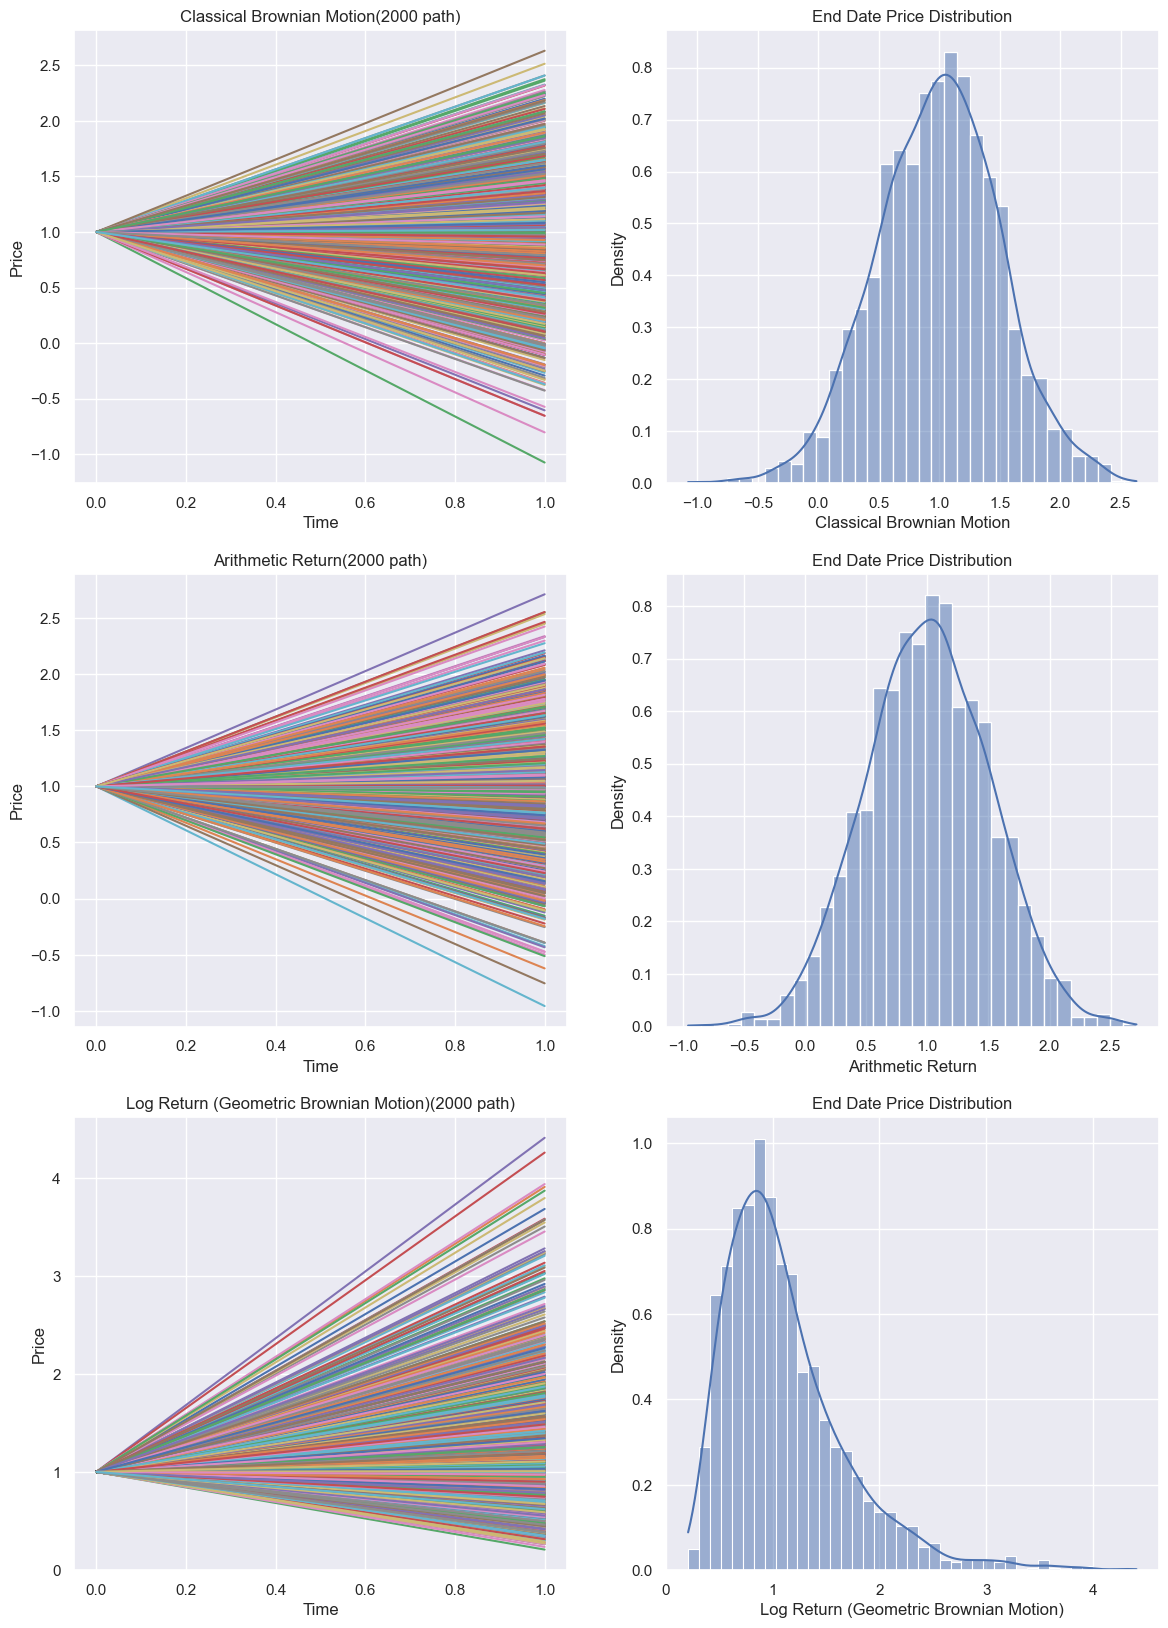
\includegraphics[width=0.9\textwidth]{./image/Problem1_1.png} 
\end{figure}

\newpage

\textbf{2. Time period > 1 (a.k.a given $P_0$ and t>1):}

Now let's make the time period larger to see what happens. We set the time period to 100, the standard deviation $\sigma$ to 0.05, the mean $\mu$ to 0, and the starting price to 1. Running the Monte Carlo 2000 times, we can see that for the Classical Brownian Motion case and the Log Return case, their estimated means and standard deviations agree with our mathematical results. However, for the Arithmetic Return case, we don't know its exact distribution, and we couldn't get the exact mean and standard deviation to compare numerically. 

If we look at the figure, we could quickly see that the closing price of the Arithmetic Return confirms our hypothesis. Its distribution is approaching a lognormal distribution. In the classical Brownian motion case, it's still normal. As to logarithmic return case, it's lognormal.

All of above results match our expectation and validate our hypothesis.

\begin{table}[htbp]
    \centering
    \caption{Time period = 100}
    \label{table2}
    \begin{tabular}{@{}ccccc@{}}
        \toprule
        \textbf{Moments} & \textbf{Items} & \textbf{Classical Brownian Motion} & \textbf{Arithmetic Return} & \textbf{Log Return}\\
        \midrule
        Mean & Estimated  & 1.00971 & 0.99468 & 1.13466 \\
        & Expected  & 1       & NAN     & 1.13315 \\
        Standard Deviation& Estimated  & 0.50361 & 0.53675 & 0.62123 \\
        & Expected & 0.5     & NAN     & 0.6039 \\
        \bottomrule
    \end{tabular}
\end{table}

\begin{figure}[htbp] 
    \centering 
    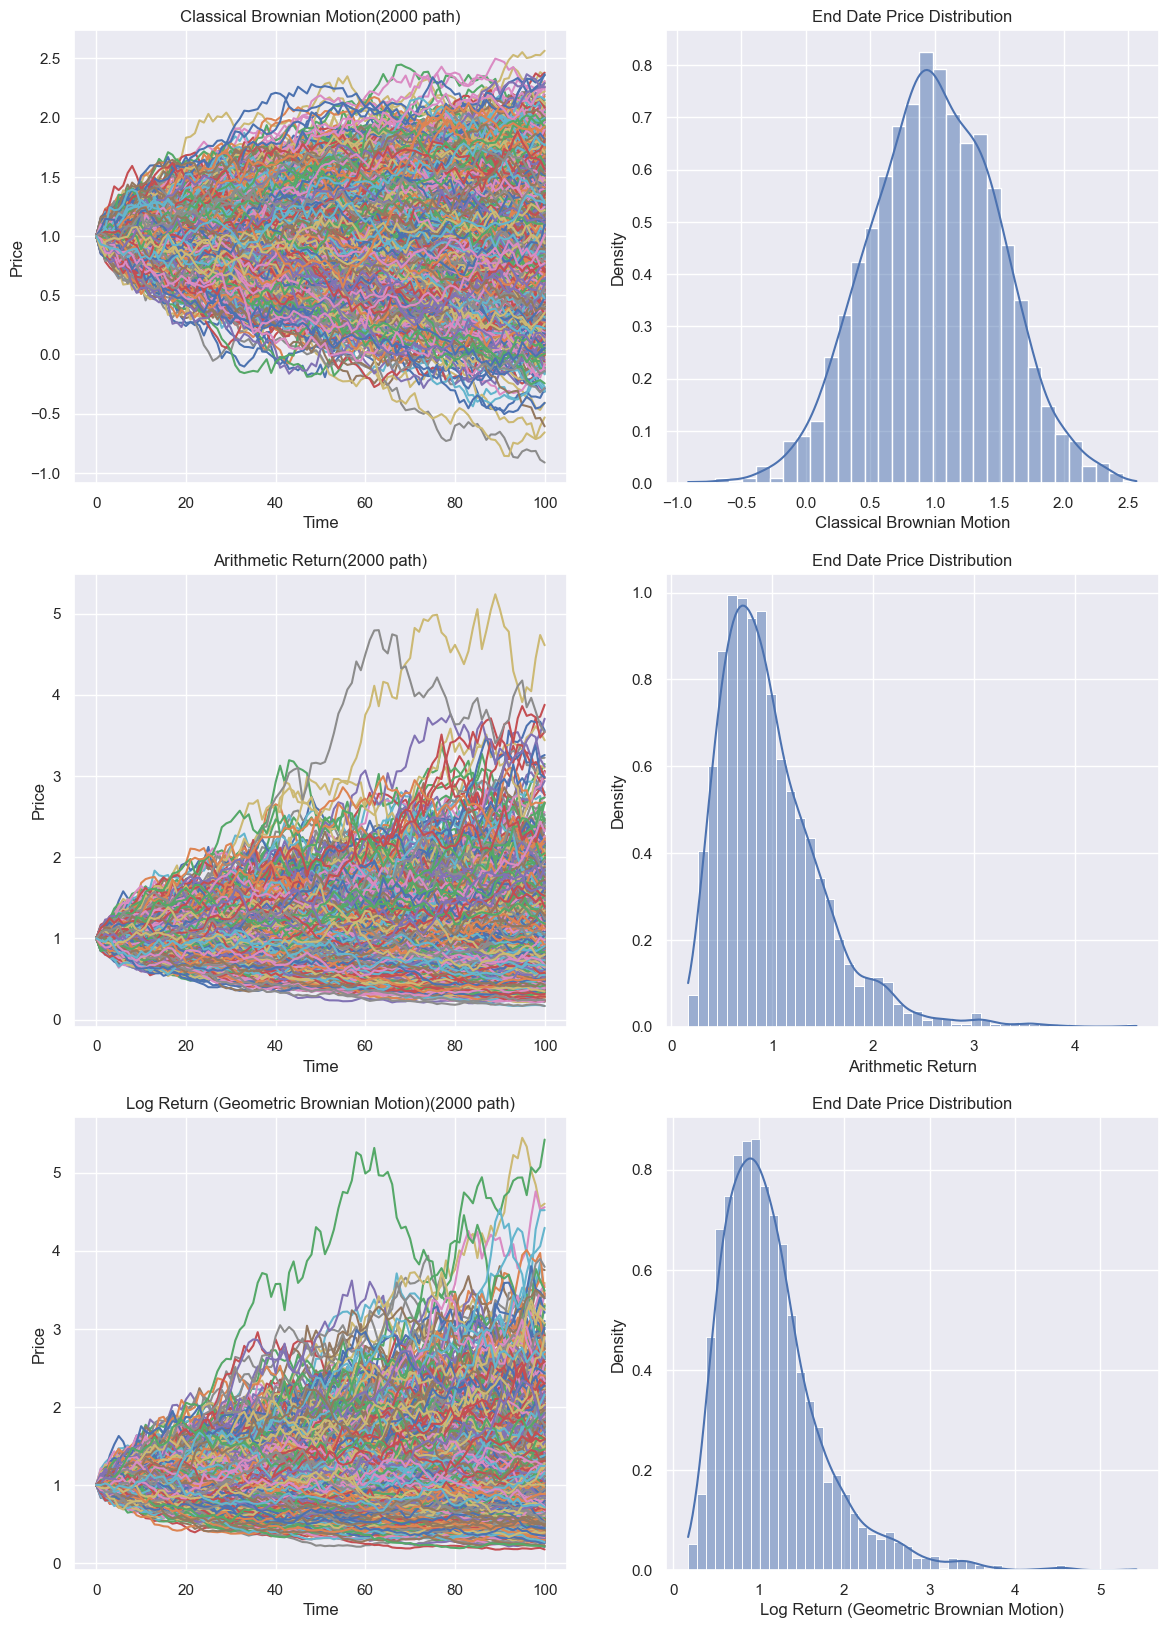
\includegraphics[width=0.9\textwidth]{./image/Problem1_2.png} 
\end{figure}



\newpage
\section*{\textcolor{orange}{Problem 2}}

Implement a function similar to the “return\_calculate\(\)” in this week's code. Allow the user to specify the method of return calculation.

Use DailyPrices.csv. Calculate the arithmetic returns for all prices.

Remove the mean from the series so that the mean(META)=0.

Calculate VaR:
\begin{enumerate}
    \item Using a normal distribution.
    \item Using a normal distribution with an Exponentially Weighted variance $\lambda$ = 0. 94
    \item Using a MLE fitted T distribution.
    \item Using a fitted AR(1) model.
    \item Using a Historic Simulation.
\end{enumerate}

Compare the 5 values.

\section*{\textcolor{orange}{Answer}}

Use return\_calculate function to get the return of each stocks then we use 5 methods to get VaR.

\subsection*{\textcolor{orange}{1. Normal Distribution}}

Assuming returns follow Normal Distribution whose mean is 0, we just need to calculate the standard deviation to understand the whole distribution. Then we get the VaR: \textbf{0.065601} or \textbf{6.5601\%} 

Compared with historical kernel density estimate, the normal returns has higher VaR and heavier tail.
\begin{figure}[htbp] 
    \centering 
    \includegraphics[width=0.6\textwidth]{./image/Normal.png} 
\end{figure}

\subsection*{\textcolor{orange}{2. normal distribution with an Exponentially Weighted variance $\lambda$ = 0. 94}}

Assuming returns follow Normal Distribution whose mean is 0, we use differnet method to calculate the standard deviation. We put more weight on cuurent information to influence the construction of volatility. Then we get the VaR: \textbf{0.091385} or \textbf{9.1385\%} 

Compared with historical kernel density estimate, the normal distribution with an Exponentially Weighted variance makes returns has much heavier tail than normal. The reason why this may happen is because we put more weight on current information and recently volatility is higher than before.

\begin{figure}[htbp] 
    \centering 
    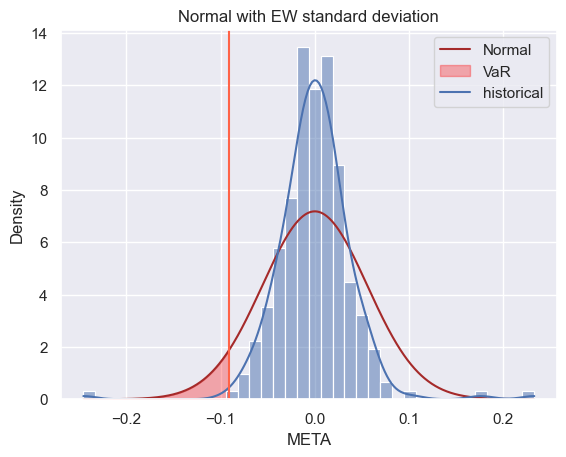
\includegraphics[width=0.6\textwidth]{./image/EWMA.png} 
\end{figure}

\subsection*{\textcolor{orange}{3. MLE fitted T distribution}}

Assuming returns follow T distribution whose mean is 0, we use MLE to estimate its degree of freedom and variance to get the whole distribution.  Then we get the VaR: \textbf{0.091385} or \textbf{9.1385\%} 

As to T distribution, it's more sharp and its tail is thinner. Its VaR is lower than above estimator.
\begin{figure}[htbp] 
    \centering 
    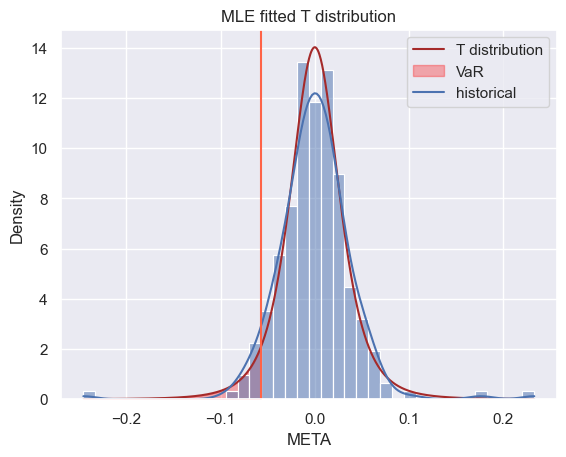
\includegraphics[width=0.6\textwidth]{./image/T.png} 
\end{figure}


\subsection*{\textcolor{orange}{4. Fitted AR(1) model}}

Assuming returns follow AR(1) model, we use MLE to estimate its cofficience of Lag 1 and variance of its error term. After finish that, then we get the VaR: \textbf{0.065705} or \textbf{6.5705\%} 

In fact, AR(1) model is normal distribution.
\[AR(1):X_t=\phi_1X_{t-1}+\varepsilon_t, \quad \{\epsilon_t\}\sim WN(0,\sigma^2)\]
\[AR(1):X_t=\varepsilon_t+\phi_1\varepsilon_t+\phi_1^2\varepsilon_t+\cdots \sim WN(0,\frac{1}{1-\varepsilon_t}\sigma^2)\]

With such knowledge, it makes sense that its curve is so similar to Normal Distribution. Also, its VaR is little higher than historical estimator.
\begin{figure}[htbp] 
    \centering 
    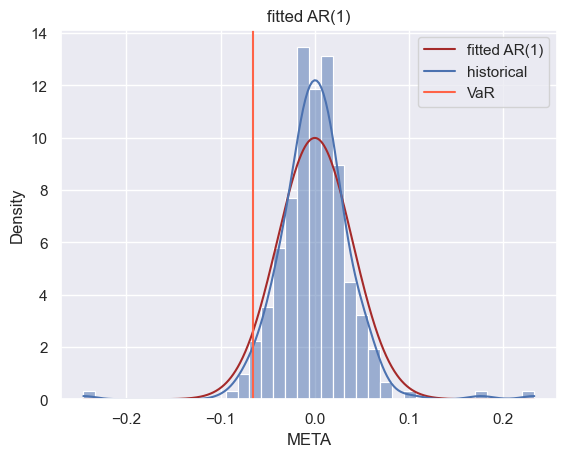
\includegraphics[width=0.6\textwidth]{./image/AR1.png} 
\end{figure}

\subsection*{\textcolor{orange}{{5. Historic Simulation}}}

 We fetch sample from the previous return data and simulate. Then then we get the VaR: \textbf{0.063881} or \textbf{6.3881\%} 

Its curve is almost same as historical kernel density estimate.
\begin{figure}[htbp] 
    \centering 
    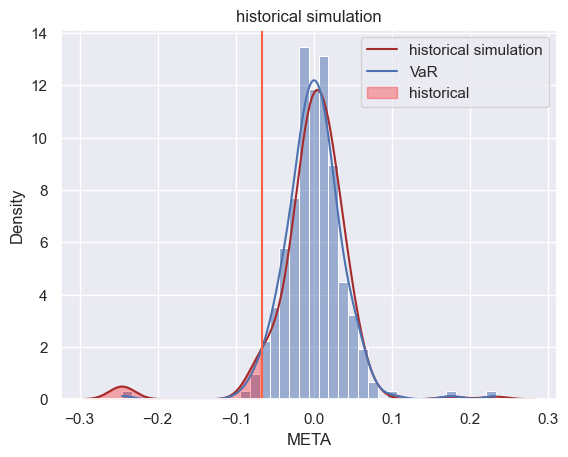
\includegraphics[width=0.6\textwidth]{./image/historic.png} 
\end{figure}

\newpage
\section*{\textcolor{orange}{Problem 3}}

Using Portfolio.csv and DailyPrices.csv. Assume the expected return on all stocks is 0.

This file contains the stock holdings of 3 portfolios. You own each of these portfolios. Using an
exponentially weighted covariance with lambda = 0.94, calculate the VaR of each portfolio as
well as your total VaR (VaR of the total holdings). Express VaR as a \$

Discuss your methods and your results.

Choose a different model for returns and calculate VaR again. Why did you choose that model? How did the model change affect the results?


\section*{\textcolor{orange}{Answer}}

\subsection*{\textcolor{orange}{1. normal distribution with an Exponentially Weighted variance $\lambda$ = 0. 94}}

We seperately calculate the VaR of Portfolio A, B, C and all of them as a whole. Let's Look at the following results:

\begin{table}[htbp]
    \centering
    \caption{VaR of Portfolio}
    \label{table3}
    \begin{tabular}{@{}ccccc@{}}
        \toprule
        \textbf{} & \textbf{portfolio A} & \textbf{portfolio B} & \textbf{portfolio C} & \textbf{Total portfolio}\\
        \midrule
        VaR & 27411.0114  & 26902.5011 & 24677.9318 & 78991.4444 \\
        \bottomrule
    \end{tabular}
\end{table}

Portfolio A has most VaR so its risk is most high. We could see from above chart that risk of A is bigger than B, C, risk of B is higher than C.

\subsection*{\textcolor{orange}{2. Historic Simulation}}

Since Historic Simulation has no assumption of the distribution of returns, its more reliable and logical.

Here is result:

\begin{table}[htbp]
    \centering
    \caption{VaR of Portfolio}
    \label{table4}
    \begin{tabular}{@{}ccccc@{}}
        \toprule
        \textbf{} & \textbf{portfolio A} & \textbf{portfolio B} & \textbf{portfolio C} & \textbf{Total portfolio}\\
        \midrule
        VaR & 10379.8217  & 9303.8174 & 8043.3187 & 28193.7417 \\
        \bottomrule
    \end{tabular}
\end{table}

It's much less than the normal distribution with an Exponentially Weighted variance. Such phenonmenon corresponds with Problem2 that
Normal Distributio with an Exponentially Weighted variance has much heavier tail.

\end{document}